\documentclass[russian]{intsys}

\usepackage{amsmath,stmaryrd,array,subcaption,xspace,algpseudocodex,minted,longtable,multirow,pifont,pgfplots,booktabs,makecell,thmtools,cite}

\usepackage{proof}
\usepackage[nottoc]{tocbibind}

\pgfplotsset{compat = 1.9}


\def\emptyset{\varnothing}
\def\phi{\varphi}
\def\psi{\varpsi}

\def\N{\mathbb{N}}
\def\V{\mathbb{V}}
\def\C{\mathbb{C}}
\def\E{\mathcal{E}}
\def\T{\mathcal{T}}
\def\O{\mathcal{O}}

\def\Rocq{\textsc{Rocq}\xspace}
\def\OCaml{\textsc{OCaml}\xspace}
\def\OCanren{\textsc{OCanren}\xspace}
\def\miniKanren{\textsc{miniKanren}\xspace}
\def\Prolog{\textsc{Prolog}\xspace}

\newcommand{\textfn}[1]{\textit{#1}}
\def\arity{\textfn{arity}\xspace}
\def\subterms{\textfn{subterms}\xspace}
\def\dom{\textfn{dom}\xspace}
\def\lhs{\textfn{lhs}\xspace}
\def\repr{\textfn{repr}\xspace}
\def\rhs{\textfn{rhs}\xspace}
\def\walk{\textfn{walk}\xspace}
\def\union{\textfn{union}\xspace}
\def\commonpart{\textfn{common\_part}\xspace}
\def\unify{\textfn{unify}\xspace}


\Author%
  {Доморацкий Эридан Алексеевич}%
  {аспирант каф. системного программирования мат.-мех. ф-та СПбГУ}%
  {Domoratskiy Eridan Alekseevich}%
  {PhD student, Software Engineering Chair, Faculty of Mathematics and Mechanics, Saint-Petersburg State University}%
  {eridan200@mail.ru}%
  {0009-0005-9020-3403}

\Author%
  {Булычев Дмитрий Юрьевич}%
  {к.ф.-м.н., доцент каф. системного программирования мат.-мех. ф-та СПбГУ}%
  {Boulytchev Dmitry Yurievich}%
  {Candidate of Physical and Mathematical Sciences, Associate Professor, Software Engineering Chair, Faculty of Mathematics and Mechanics, Saint-Petersburg State University}%
  {dboulytchev@math.spbu.ru}%
  {0000-0001-8363-7143}

\TitleRU{Эффективная персистентная унификация рациональных термов}
\ShortTitle{Эффективная рациональная унификация}
\AbstractRU{%
  В работе исследуется производительность алгоритмов для решения задачи синтаксической унификации возможно-бесконечных термов
  первого порядка с конечным числом различных подтермов (рациональных термов). Показано, что наиболее распространённый на практике
  алгоритм Юэ для решения данной задачи не является наилучшим в персистентных условиях. Описан алгоритм, который показывает более высокую
  производительность не только в персистентной реализации, но и в эфемерной реализации при некоторых экстремальных входных параметрах.
}
\KeywordsRU{персистентные алгоритмы, рациональные деревья, унификация, логическое программирование}

\TitleEN{An Efficient Persistent Unification for Rational Terms}
\AbstractEN{%
  The paper studies the performance of algorithms for rational terms syntactic unification. We show that a well-known Huet's algorithm
  is inappropriate in persistent settings, and devise another one which performs better. On some extremal inputs our algorithm wins
  even in ephemeral implementaion.
}
\KeywordsEN{persistent algorithms, rational tree, unification, relational programming}


\begin{document}

\section{Введение}

Основной операцией чистого логического программирования является синтаксическая унификация~\cite{robinson1965machine} термов первого порядка (они же эрбрановы деревья). Унификация позволяет решать уравнения между термами за счёт уточнения их свободных переменных. Синтаксическая унификация отличается тем, что любые функциональные символы полагаются неинтерпретируемыми -- то есть, применение функционального символа к термам $f\,(t_1, ..., t_n)$ интерпретируется как идентичная синтаксическая конструкция. Все такие конечные синтаксические записи образуют эрбранову вселенную, адекватность применения которой обосновывается теоремой Эрбрана~\cite{herbrand1930}.

Помимо логического программирования, синтаксическая унификация находит применение при выводе и проверке типов в языках программирования. В зависимости от конкретной системы типов, иногда полезно расширить пространство возможных синтаксических форм бесконечными -- это позволяет говорить о рекурсивных типах (например, в языке программирования \OCaml~\cite{gauthier2004numbering}). Тем не менее, произвольно-бесконечные термы не имеют практической применимости в вычислительной математической логике, потому что для их порождения потребовалось бы затратить бесконечное время работы программы. Вместо этого рассматривают более узкий класс возможно-бесконечных термов -- рациональные термы. Рациональным термом~\cite{colmerauer1982prolog} называют такой возможно-бесконечный терм, множество подтермов (в смысле поддеревьев) которого конечно. В частности, любой рекурсивный тип можно представить как рациональный терм.

В логическом программировании унификация рациональных термов также находит применение, но не столько за её выразительную способность, сколько за скорость работы. Проблема в том, что для ограничения конечности термов требуется выполнение трудоёмкой\footnote{Например, реализация конкатенации двух списков при использовании классического алгоритма унификации требует затрат $\mathcal{O}(n^2)$ времени вместо $\mathcal{O}(n)$~\cite{colmerauer1982prolog}.} <<проверки вхождения>> (англ. <<occurs check>>) или применение более сложных алгоритмов унификации~\cite{martelli1982efficient}, обладающих непрактичными накладными расходами времени работы. Из-за этого практические реализации языков логического программирования (например, SWI-Prolog) используют унификацию рациональных термов, позволяя пользователю в частных случаях проверять отсутствие зацикливания внутри термов.

Несмотря на то, что рациональная унификация является хорошо изученной темой, в рамках которой было предложено множество алгоритмов~\cite{huet1976resolution,mukai1983unification,martelli1984efficient,jaffar1984efficient}, обширное применение получил только первый из перечисленных алгоритм Юэ~\cite{huet1976resolution}. Оптимальная реализация данного алгоритма действительно хорошо работает в существующих приложениях за счёт использования изменяемой памяти. В реализациях языка \Prolog это возможно благодаря использованию WAM (Warren Abstract Machine~\cite{warren1983abstract}), которая реализует поиск в глубину с откатами -- то есть, при ошибке в активной ветке дерева поиска выполняется откат состояний изменяемых переменных в памяти до ближайшего ветвления (backtracking). А в выводе типов основной упор делается на детерминированность поиска -- то есть, если произошла ошибка, нет смысла рассматривать никакие альтернативные ветки.

Тем не менее, в логическом программировании выделяют отдельную область реляционного программирования и язык \miniKanren~\cite{friedman2005reasoned}. Одним из отличий \miniKanren от \Prolog является использование поиска с перестановками (interleaving search~\cite{kiselyov2005backtracking}) вместо поиска в глубину. Такой выбор обусловлен полнотой поиска -- способностью находить все возможные решения за некоторое конечное время, -- в отличие от поиска в глубину, который может уйти в непродуктивный бесконечный цикл. Для реализации поиска с перестановками обычно используют персистентные структуры данных для представления отдельных состояний в дереве поиска, потому что процедура поиска вынуждена <<одновременно>> поддерживать несколько <<активных>> состояний, переключение между которыми может выполняться неожиданным образом.

В этой работе мы описываем собственный алгоритм для унификации рациональных термов на основе подхода Мартелли и Росси~\cite{martelli1984efficient}. Наш алгоритм обладает доказанной корректностью и завершаемостью, формально верифицированными в системе автоматической проверки доказательств \Rocq. Сами доказательства не являются предметом данной статьи, но в тексте мы иногда ссылаемся на конкретные определения из реализации на \Rocq\footnote{\url{https://github.com/dboulytchev/miniKanren-coq/tree/master/src/Rational}}.

Основным результатом этой работы является экспериментальный анализ производительности нашего алгоритма и алгоритма Юэ~\cite{huet1976resolution} в сравнении с классическим алгоритмом Робинсона с треугольными подстановками~\cite{baader2001unification}. Представленный анализ показывает, что в практических сценариях наш алгоритм обходит по скорости алгоритм Юэ будучи реализованным персистентно, хотя и уступает в эфемерной (не персистетной) реализации. В то же время нам удалось показать, что существуют сценарии, когда алгоритм Юэ работает значительно (более, чем константно) медленнее нашего.


\subsection{Рациональные термы}

Пусть заданы счётно-бесконечные множества переменных $x, y, z, ... \in \V$ и конструкторов (функциональных символов) $f, g, h, ... \in \C$, а также функция $\arity : \C \rightarrow \N$, определяющая арности конструкторов. Для удобства, мы используем запись $f^n \in \C$, где $f \in \C$, а $n = \arity(f)$.

Определим отображение $F : \text{Set} \rightarrow \text{Set}$, и множества термов $T = \mu F$ и (возможно-)бесконечных термов $T^\infty = \nu F$ как наименьшую и наибольшую~\cite{simon2006coinductive} неподвижные точки этого отображения соответственно:
\[F(X) = \V \cup \{ f^n\,(t_1, ..., t_n) \mid f^n \in \C, t_i \in X \}.\]
Множество подтермов $\subterms : T^\infty \rightarrow 2^{T^\infty}$ определяется индуктивно:
\begin{itemize}
    \item $t \in \subterms(t)$;
    \item $t \in \subterms(t_i) \implies t \in \subterms(f^n\,(..., t_i, ...))$.
\end{itemize}
Тогда множество рациональных термов определяется как:
\[T^R = \{ t \in T^\infty \mid \subterms(t) \text{ конечно} \}.\]
Естественно, что $T \subset T^R \subset T^\infty$, поэтому многие определения даются для $T^\infty$ и автоматически действуют для $T$ и $T^R$.

Подстановкой $\sigma \in \Sigma$ мы называем такое отображение $\V \rightarrow T^\infty$, которое обладает конечным доменом подстановки $\dom(\sigma) = \{ x \in \V \mid \sigma(x) \neq x \}$. Применением подстановки $\sigma$ к терму $t \in T^\infty$ называется гомоморфное расширение применения подстановки как функции и записывается в постфиксной форме как $t \sigma$:
\begin{equation*}
    \begin{array}{r@{{}={}}l}
        x \sigma & \sigma(x) \\
        f^n\,(..., t_i, ...) \sigma & f^n\,(..., t_i \sigma, ...) \\
    \end{array}
\end{equation*}

\section{Описание алгоритма}

Описанный далее алгоритм основан на алгоритме <<UNIFY-1>>, представленном в работе Мартелли и Росси~\cite{martelli1984efficient}. По сравнению с ним, наш алгоритм специализирован для обработки одного уравнения за раз, что зачастую и требуется на практике, вместо обработки заранее заданного множества уравнений. Это позволило упростить описание структур данных и самого алгоритма, приблизив их к практической реализации.

\subsection{Система уравнений}

Несмотря на то, что понятие системы уравнений обладает общепринятым определением, в данной работе мы так называем объект, получаемый в результате работы нашего алгоритма.

Для некоторого множества $A$ введём обозначение $A^? = \{ \bot \} \cup A$, которое мы называем <<опциональный $A$>>.

\begin{definition}[Уравнение]
    Назовём \textit{уравнением} $e \in \E$ упорядоченную пару из:
    \begin{enumerate}
        \item множества переменных <<левая сторона>> с отмеченной точкой <<представляющая переменная>>;
        \item опционального (конечного) терма <<правая сторона>>, не являющегося переменной.
    \end{enumerate}

    Для удобства мы вводим проекции $\lhs : \E \rightarrow 2^\V$, $\repr : \E \rightarrow \V$ и $\rhs : \E \rightarrow T^?$ для левой стороны, представляющей переменной и правой стороны уравнения соответственно. Также, мы используем нотацию $\underline{x}, y, z \equiv t$ для обозначения уравнения, в котором $\lhs(\underline{x}, y, z \equiv t) = \{ x, y, z \}$, $\repr(\underline{x}, y, z \equiv t) = x$ и $\rhs(\underline{x}, y, z \equiv t) = t$.
\end{definition}

\begin{definition}[Система уравнений]
    Назовём \textit{системой уравнений} $\xi \in \Xi$ конечное множество уравнений с попарно непересекающимися левыми сторонами. Для удобства мы будем обозначать пополнение системы уравнений новым уравнением $e$ как $\xi, e$:
    \[\{ e \} \cup \{ e' \in \xi \mid \lhs(e) \cap \lhs(e') = \emptyset \}.\]
\end{definition}

Данное определение уравнения стоит рассматривать как частный случай системы уравнений в общепринятом смысле. Например:
\begin{equation*}
    \begin{array}{c|c}
        \text{Общепринятая система уравнений} & \text{Наше уравнение} \\[2pt]
        \left\{\begin{array}{l@{{}={}}l}
            x & f\,(z) \\
            y & x \\
            z & x \\
        \end{array}\right. & \underline{x}, y, z \equiv f\,(z) \\
    \end{array}
\end{equation*}

В этом смысле тривиальные уравнения вида $\underline{x} \equiv \bot$ <<ничего не уравнивают>>, поэтому мы дополнительно считаем, что никакая система уравнений $\xi \in \Xi$ не может содержать таких уравнений:
\[\forall x \in \V, \xi \in \Xi. ~ \underline{x} \equiv \bot \notin \xi.\]

Мы определяем две операции на системах уравнений. Основная операция $\walk : \Xi \times \V \rightarrow \E \times T$ по данной системе уравнений и переменной находит соответствующее уравнение:
\begin{equation*}
    \walk(\xi, x) = \begin{cases}
        (e, \rhs(e)) & \text{если $e \in \xi, x \in \lhs(e)$ и $\rhs(e) \neq \bot$}, \\
        (e, \repr(e)) & \text{если $e \in \xi, x \in \lhs(e)$ и $\rhs(e) = \bot$}, \\
        (\underline{x} \equiv \bot, x) & \text{иначе}. \\
    \end{cases}
\end{equation*}

С помощью этой операции можно определить отображение $\llbracket \cdot \rrbracket : \Xi \rightarrow \Sigma$, задающее интерпретацию системы уравнений как подстановки. Результат применения $t \llbracket \xi \rrbracket$ задаётся следующим псевдокодом:
\begin{algorithmic}
    \Function{ApplyEqSys}{$\xi \in \Xi$, $t \in T^\infty$}
        \If{$x \gets t \in \V$}
            \State $(\_, t) \gets \walk(\xi, x)$
        \EndIf
        \If{$x' \gets t \in \V$}
            \State \Return $x'$
            \Comment{неподвижная точка}
        \EndIf
        \If{$f^n\,(t_1, \dots, t_n) \gets t$}
            \State \Return $f^n\,(\Call{ApplyEqSys}{\xi, t_1}, \dots, \Call{ApplyEqSys}{\xi, t_n})$
        \EndIf
    \EndFunction
\end{algorithmic}

\begin{theorem}
    Для любых $\xi \in \Xi$ и $t \in T^R$ верно, что $t \llbracket \xi \rrbracket \in T^R$.
\end{theorem}
\begin{proof}
    Достаточно заметить, что уравнений в системе конечное число и их правые стороны также конечны. Более подробно см. \texttt{wf\_eqsys\_to\_subst\_rational} и \texttt{inf\_subst\_apply\_rational} в реализации на \Rocq.
\end{proof}

Вторая вводимая операция $\union : \Xi \times \V \times \V \rightarrow \Xi \times (T \times T)^?$ преобразует данную систему уравнений так, чтобы данные переменные лежали в одном уравнении:
\begin{algorithmic}[1]
    \Function{UnionEqSys}{$\xi \in \Xi$, $x, y \in \V$}
        \State $(e_x, \_) \gets \walk(\xi, x)$
        \State $(e_y, \_) \gets \walk(\xi, y)$
        \If{$\repr(e_x) = \repr(e_y)$}
            \State \Return $(\xi, \bot)$
            \Comment{уже лежат в одном уравнении или равны}
        \EndIf
        \If{$\rhs(e_x) = \bot$ \textbf{and} $\rhs(e_y) = \bot$}
            \State \Return $([\xi, \lhs(e_x) \cup \lhs(e_y) \equiv \bot], \bot)$
        \EndIf
        \If{$\rhs(e_x) = \bot$}
            \State \Return $([\xi, \lhs(e_x) \cup \lhs(e_y) \equiv \rhs(e_y)], \bot)$
        \EndIf
        \If{$\rhs(e_y) = \bot$}
            \State \Return $([\xi, \lhs(e_x) \cup \lhs(e_y) \equiv \rhs(e_x)], \bot)$
        \EndIf
        \State \Return $([\xi, \lhs(e_x) \cup \lhs(e_y) \equiv \rhs(e_x)],(\rhs(e_x), \rhs(e_y)))$ \\
        \Comment{конфликт правых сторон уравнений}
    \EndFunction
\end{algorithmic}

В приведённом псевдокоде, когда добавляется новое уравнение на строках 6-12, мы можем выбрать в качестве представляющей переменной как $\repr(e_x)$, так и $\repr(e_y)$ -- это не влияет на теоретические свойства алгоритма. То же верно и про выбор правой стороны добавляемого уравнения на строке 12: это может быть как $\rhs(e_x)$, так и $\rhs(e_y)$. Как показывает псевдокод, второе возвращаемое значение сигнализирует о конфликте правых сторон. Квадратные скобки используются для группировки и не несут специального смысла.


\subsection{Общая часть термов}

Одной из важных частей алгоритма является операция выделения <<общей части>>~\cite{martelli1984efficient} двух конечных термов, $\commonpart : T \times T \rightarrow T^?$:
\begin{equation*}
    \begin{split}
        \commonpart(x, \_) &= x \\
        \commonpart(\_, y) &= y \\
        \commonpart(f^n\,(..., l_i, ...), f^n\,(..., r_i, ...)) &= f^n\,(..., \commonpart(l_i, r_i), ...) \\
    \end{split}
\end{equation*}

Мы задаём поведение этой функции в стиле индуктивного предиката. Такое определение удобно, потому что оставляет некоторую свободу в выборе результата, когда функция применяется к двум переменным -- можно выбрать любую из них. В случаях, когда никакое из правил не подходит, полагается значение $\bot$.


\subsection{Алгоритм}

Алгоритм задаётся рекурсивной функцией $\unify : \Xi \times T \times T \rightarrow \Xi^?$:
\begin{algorithmic}[1]
    \Function{RationalUnify}{$\xi \in \Xi$, $t_1, t_2 \in T$}
        \If{$x \gets t_1 \in \V$ \textbf{and} $y \gets t_2 \in \V$}
            \State $(\xi, ts) \gets \union(\xi, x, y)$
            \If{$(t_1, t_2) \gets ts$}
                \State \Return $\Call{RationalUnify}{\xi, t_1, t_2}$
                \Comment{разрешение конфликта}
            \EndIf
            \State \Return $\xi$
        \EndIf
        \If{$x \gets t_1 \in \V$}
            \State $(e, \_) \gets \walk(\xi, x)$
            \If{$\rhs(e) = \bot$}
                \State \Return $\xi, \lhs(e) \equiv t_2$
            \EndIf
            \State $t \gets \commonpart(\rhs(e), t_2)$
            \If{$t = \bot$}
                \State {\bf failure}
            \EndIf
            \State $\xi \gets \xi, \lhs(e) \equiv t$
            \Comment{упрощение правой стороны уравнения}
            \State \Return \Call{RationalUnify}{$\xi, \rhs(e), t_2$}
        \EndIf
        \If{$y \gets t_2 \in \V$}
            \State \Return \Call{RationalUnify}{$\xi, y, t_1$}
        \EndIf
        \If{$f^n\,(l_1, ..., l_n) \gets t_1$ \textbf{and} $g^m\,(r_1, ..., r_m) \gets t_2$}
            \If{$f^n \neq g^m$}
                \State \bf failure
            \EndIf
            \For{$i = 1, ..., n$}
                \State $\xi \gets \Call{RationalUnify}{\xi, l_i, r_i}$
            \EndFor
            \State \Return $\xi$
        \EndIf
    \EndFunction
\end{algorithmic}

\begin{theorem}[Корректность]
    Алгоритм \textsc{RationalUnify} корректен.
\end{theorem}
\begin{proof}
    Точная формулировка корректности и доказательство (индукция по дереву вывода) выходят за рамки данной статьи, но приведены в реализации на \Rocq под названиями \texttt{rational\_unification\_correct} и \texttt{rational\_unification\_complete}.
\end{proof}

\begin{theorem}[Завершаемость]
    Для любых $\xi \in \Xi$ и $t_1, t_2 \in T$ алгоритм \textsc{RationalUnify} завершается с некоторым результатом.
\end{theorem}
\begin{proof}
    Фундированная (well-founded) индукция по <<размеру>> входных параметров алгоритма. См. \texttt{rational\_unification\_exists} в реализации на \Rocq.
\end{proof}

\section{Реализация алгоритма}

Полноценная реализация алгоритма со всеми оптимизациями требует значительного количества кода, поэтому в этом разделе описаны только основные подходы. Для простоты примеры кода приводятся на языке программирования \OCaml.

Предположим, что термы заданы следующим алгебраическим типом данных:
\begin{minted}{OCaml}
type term =
| Var of int
| Con of int * term array
\end{minted}


\subsection{Система уравнений}

По аналогии с треугольными подстановками~\cite{baader2001unification}, наши системы уравнений естественным образом представляются в <<треугольном>> виде. Для этого мы используем тип частичных отображений из номеров переменных в термы \mintinline{OCaml}|term M.t|:
\begin{minted}{OCaml}
module M = Map.Make(Int)
\end{minted}

Во всех операциях над системами уравнений, мы используем номера представляющих переменных вместо $\E$. Таким образом, \walk реализуется следующим образом:
\begin{minted}{OCaml}
let rec walk s x = match M.find x s with
| exception Not_found -> x, Var x
| Var x -> walk s x
| t -> x, t
\end{minted}

Простейшая реализация операции \union, соответственно:
\begin{minted}{OCaml}
let union s x y =
  let x, xt = walk s x in
  let y, yt = walk s y in
  if x == y then s, None
  else begin match xt, yt with
  | Var _, Var _ -> M.add x yt s, None
  | Var _, _ -> M.add x (Var y) s, None
  | _, Var _ -> M.add y (Var x) s, None
  | _, _ -> M.add x (Var y) s, Some (xt, yt)
  end
\end{minted}

На практике, при реализации \union стоит применять эвристику <<возраста переменных>>~\cite{mannila1986complexity}: по возможности связывать <<более свежие>> переменных (обладающие б\'{о}льшими номерами) с <<менее свежими>>. Обоснование данной эвристики описано в процитированной статье, но на практике она позволяет уменьшить глубину рекурсии \walk подобно тому, как это делает ранговая эвристика в структуре данных СНМ (система непересекающихся множеств~\cite{galler1964improved}). Примеры реализации с использованием этой оптимизации приведены в репозитории с анализом производительности алгоритма.


\subsection{Общая часть термов}

Простейшая реализация \commonpart повторяет определение:
\begin{minted}{OCaml}
let rec common_part x y = match x, y with
| Var x, _ -> Var x
| _, Var y -> Var y
| Con (f, ts1), Con (g, ts2)
when f == g && Array.length ts1 == Array.length ts2 ->
  Con (f, Array.map2 common_part ts1 ts2)
| _ -> raise No_common_part
\end{minted}

На практике, полезно, чтобы реализация \commonpart возвращала непосредственно один из своих аргументов всегда, когда это возможно. Это позволяет снизить затраты памяти и увеличить шанс срабатывания быстрой проверки по равенству ссылок (<<physical equality>>) при выполнении унификации.

Для этого можно рассмотреть следующую решётку из четырёх элементов (<<сторона>>, \textsf{Side}): $\top$, $\Leftarrow$, $\Rightarrow$ и $\bot$.
\begin{center}
    \begin{tikzpicture}
        \node (both) at (0, 1) {$\top$};
        \node (left) at (-1, 0) {$\Leftarrow$};
        \node (right) at (1, 0) {$\Rightarrow$};
        \node (aside) at (0, -1) {$\bot$};
        \draw[dotted] (left) -- (both) node[midway,sloped] {$<$};
        \draw[dotted] (right) -- (both) node[midway,sloped] {$>$};
        \draw[dotted] (aside) -- (left) node[midway,sloped] {$>$};
        \draw[dotted] (aside) -- (right) node[midway,sloped] {$<$};
        \node[anchor=south] at (both.north) {<<обе>>};
        \node[anchor=east] at (left.west) {<<слева>>};
        \node[anchor=west] at (right.east) {<<справа>>};
        \node[anchor=north] at (aside.south) {<<ни одна>>};
    \end{tikzpicture}
\end{center}

Тогда можно реализовать обобщённую функцию $\commonpart' : T \times T \rightarrow (T \times \textsf{Side})^?$, которая вторым возвращаемым параметром в случае успеха дополнительно сообщает, какие из аргументов подходят на роль результата. Нерекурсивные вызовы в реализации очевидны, а при рекурсивных вызовах требуется накапливать инфинум <<сторон>>:
\begin{itemize}
    \item Если накопленный инфинум -- $\bot$, функция вынуждена вернуть сконструированный терм, потому что никакой из аргументов не подходит на роль результата.
    \item Иначе -- отбросить сконструированный терм и вернуть тот аргумент, на который указывает накопленный инфинум.
\end{itemize}

Конкретные примеры реализации расположены в репозитории с анализом производительности.


\subsection{Алгоритм}

Наконец, реализация \unify почти полностью повторяет псевдокод:
\begin{minted}{OCaml}
let rec unify_vt s x yt =
  let x, xt = walk s x in
  begin match xt with
  | Var _ -> M.add x yt s
  | _ ->
    let t = common_part xt yt in
    unify (M.add x t s) xt yt
  end

and unify s xt yt =
  if xt == yt then s
  else match xt, yt with
  | Var x, Var y ->
    begin match union s x y with
    | s, Some (xt, yt) -> unify s xt yt
    | s, None -> s
    end
  | Var x, _ -> unify_vt s x yt
  | _, Var y -> unify_vt s y xt
  | Con (f, ts1), Con (g, ts2)
  when f == g && Array.length ts1 == Array.length ts2 ->
    let n = Array.length ts1 in
    let rec hlp i s =
      if i == n then s
      else hlp (i + 1) @@ unify s ts1.(i) ts2.(i)
    in
    hlp 0 s
  | _ -> raise No_common_part
\end{minted}

\section{Анализ производительности}

Мы реализовали три алгоритма на языке программирования \OCaml\footnote{\url{https://github.com/ProgMiner/rational-unification}}:
\begin{itemize}
    \item \texttt{robinson}~--- алгоритм Робинсона с <<треугольными>> подстановками~\cite{baader2001unification};
    \item \texttt{rational}~--- наш алгоритм, описанный выше;
    \item \texttt{huet}~--- алгоритм Юэ~\cite{huet1976resolution} на основе реализации в SWI-Prolog\footnote{\url{https://github.com/SWI-Prolog/swipl/blob/45e83178379f0fd6f918bd294bb361f3db7bf1d7/src/pl-prims.c\#L71}}.
\end{itemize}

Все три алгоритма были реализованы в двух вариантах: эфемерном (с изменяемыми переменными) и персистентном. Дополнительно были реализованы эфемерные варианты алгоритмов со сжатием путей. Для справедливого сравнения все реализации выполнены с наиболее подходящими структурами данных и оптимизированы насколько это было возможно.

Для тестирования использовались <<трассы унификации>>. Каждая трасса представляет собой список уравнений, где каждое уравнение задано парой термов. Всего было подготовлено три набора тестов:
\begin{itemize}
    \item \texttt{JGS}~--- собраны автоматически из тестов <<Java Generic Solver>>~\cite{lozov2023relational} (9 тестов, 1448 трасс);
    \item \texttt{Lama}~--- собраны автоматически из тестов <<Lama type checker>>~\cite{domoratskiy2024relational} (66 трасс, по одной на тест);
    \item \texttt{synth}~--- синтетические тесты, сгенерированны вручную (66 трасс, по 11 на тест).
\end{itemize}

Мы считаем наборы тестов \texttt{JGS} и \texttt{Lama} близкими к прикладным задачам унификации <<из реального мира>>. Для выполнения трасс из набора \texttt{JGS} достаточно классической унификации (конечных термов), тогда как некоторые трассы из набора \texttt{Lama} требуют поддержки рациональной унификации.

Синтетические тесты были подобраны эмпирически для нагрузочного тестирования алгоритмов. Каждый из перечисленных тестов параметризован числом $n = 0, 10, ..., 100$:
\begin{itemize}
    \item \texttt{full}~--- уравнивает два полных двоичных дерева глубины $n$ ($T_i, U_i \in \V$):
    \begin{equation*}
        \left\{
        \begin{array}{c@{{}={}}ll}
            T_0 & x, & x \in \V, \\
            U_0 & a, & a^0 \in \C, \\
            T_i & f\,(T_{i-1}, T_{i-1}), & i = 1, 2, \dots, n, \\
            U_i & f\,(U_{i-1}, U_{i-1}), & i = 1, 2, \dots, n, \\
            T_n & U_n. \\
        \end{array}
        \right.
    \end{equation*}
    \item \texttt{left\_right}~--- уравнивает <<левостороннее>> и <<правостороннее>> двоичные деревья глубины $n$ ($T_i, U_i \in \V$):
    \begin{equation*}
        \left\{
        \begin{array}{c@{{}={}}ll}
            T_0 & x, \\
            U_0 & x, \\
            T_i & f\,(T_{i-1}, x), & i = 1, 2, \dots, n, \\
            U_i & f\,(x, U_{i-1}), & i = 1, 2, \dots, n, \\
            T_n & U_n. \\
        \end{array}
        \right.
    \end{equation*}
    \item $\texttt{loops}_1$~--- уравнивает $n$ <<петель>> друг с другом:
    \begin{equation*}
        \left\{
        \begin{array}{c@{{}={}}ll}
            x_i & f\,(x_i), & i = 1, 2, \dots, n, \\
            x_0 & x_i, & i = 1, 2, \dots, n. \\
        \end{array}
        \right.
    \end{equation*}
    \item $\texttt{loops}_2$ --- как предыдущий, но с $x_i = x_0$ вместо $x_0 = x_i$.
    \item $\texttt{loops}_3$ --- как $\texttt{loops}_1$, но с $x_{i-1} = x_i$ вместо $x_0 = x_i$.
    \item $\texttt{loops}_4$ --- как предыдущий, но с $x_i = x_{i-1}$ вместо $x_{i-1} = x_i$.
\end{itemize}

Все синтетические тесты, кроме \texttt{full}, требуют поддержки рациональной унификации. Тем не менее, тест \texttt{full} затрачивает экспоненциальное количество времени и памяти при запуске на алгоритме Робинсона. По этой причине, синтетические тесты использовались только для сравнения алгоритмов рациональной унификации между собой.

Замеры проводились на компьютере под управлением ОС Alpine Linux с изоляцией одного ядра процессора (13th Gen Intel® Core™ i7-1360P) и прикреплением тестирующего процесса к выделенному ядру\footnote{\url{https://github.com/ProgMiner/bench-linux}}. Все промежуточные результаты замеров приведены в упомянутом ранее репозитории и могут быть воспроизведены.

Основные результаты сравнения:
\begin{itemize}
    \item Наш алгоритм работает настолько же быстро, насколько и классический алгоритм Робинсона в <<реальных>> сценариях использования, что продемонстрировано на \autoref{fig:baseline}. Приведённые графики отражают время работы алгоритмов рациональной унификации по отношению ко времени работы алгоритма Робинсона. В частности, на графиках видно, что наш алгоритм в обоих случаях держится вблизи главной диагонали.
    \item Несмотря на то, что алгоритм Юэ работает быстрее в эфемерной реализации, он деградирует будучи реализованным персистентно~--- это отражено как на \autoref{fig:baseline}, так и на \autoref{fig:Lama}. Более того, \autoref{fig:synth-ephemeral} и \autoref{fig:synth-persistent} также демонстрируют, что в некоторых случаях алгоритм Юэ начинает работать значительно медленнее даже в эфемерной реализации, а также, что время его работы зависит от порядка сторон уравнений (разница между $\texttt{loops}_1$ и $\texttt{loops}_2$).
\end{itemize}

\begin{figure}[t]
    \centering
    \begin{subfigure}{.48\linewidth}
        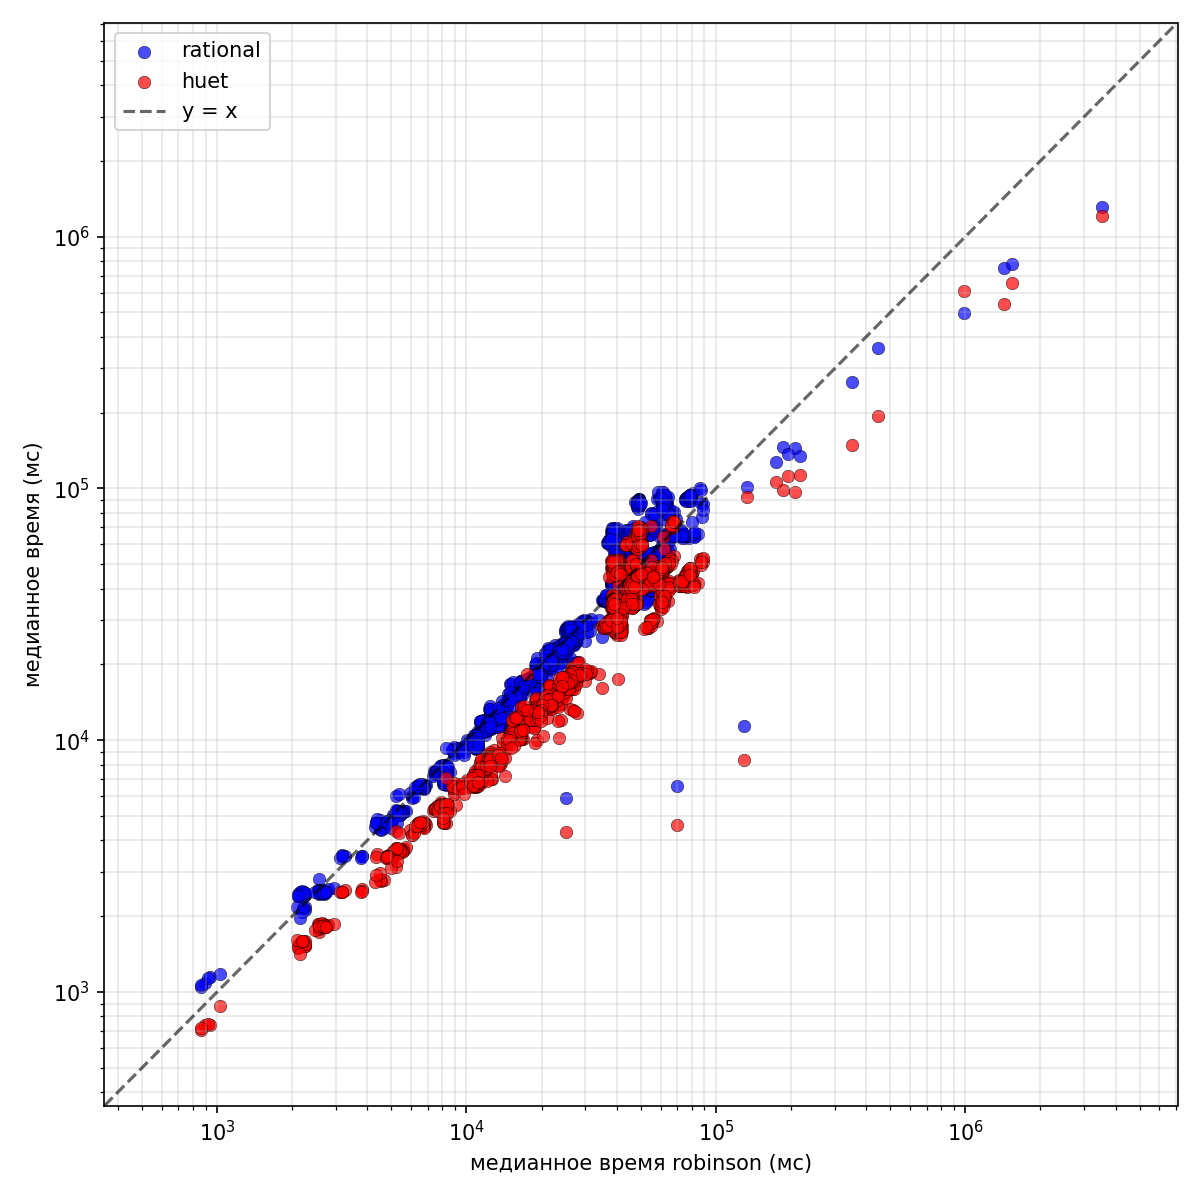
\includegraphics[width=\linewidth]{bench/ephemeral/robinson_comparison.png}
        \subcaption{Эфемерная реализация}
    \end{subfigure}
    \hfill
    \begin{subfigure}{.48\linewidth}
        
\includegraphics[width=\linewidth]{bench/persistent/robinson_comparison.png}
        \subcaption{Персистентная реализация}
    \end{subfigure}
    \caption{Сравнение производительности алгоритмов рациональной унификации по отношению к алгоритму Робинсона.}
    \label{fig:baseline}
\end{figure}

\begin{figure}[b]
    \centering
    \begin{subfigure}{.48\linewidth}
        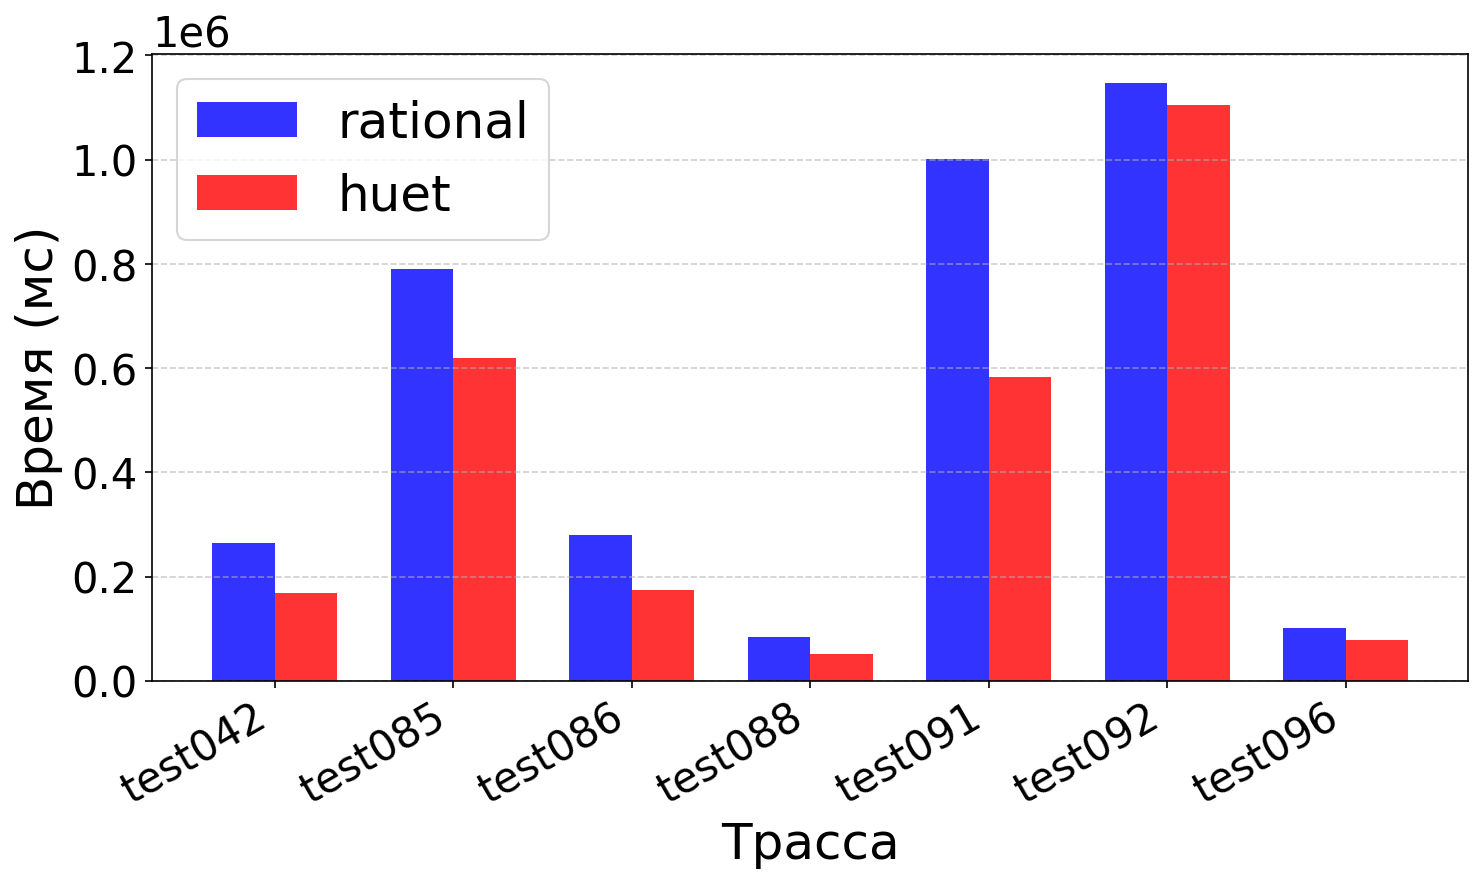
\includegraphics[width=\linewidth]{bench/ephemeral/Lama.png}
        \subcaption{Эфемерная реализация}
    \end{subfigure}
    \hfill
    \begin{subfigure}{.48\linewidth}
        
\includegraphics[width=\linewidth]{bench/persistent/Lama.png}
        \subcaption{Персистентная реализация}
    \end{subfigure}
    \caption{Сравнение алгоритмов на трассах \texttt{Lama}, которые требуют поддержки рациональной унификации}
    \label{fig:Lama}
\end{figure}

\begin{figure}[p]
    \centering
    \begin{subfigure}{.48\linewidth}
        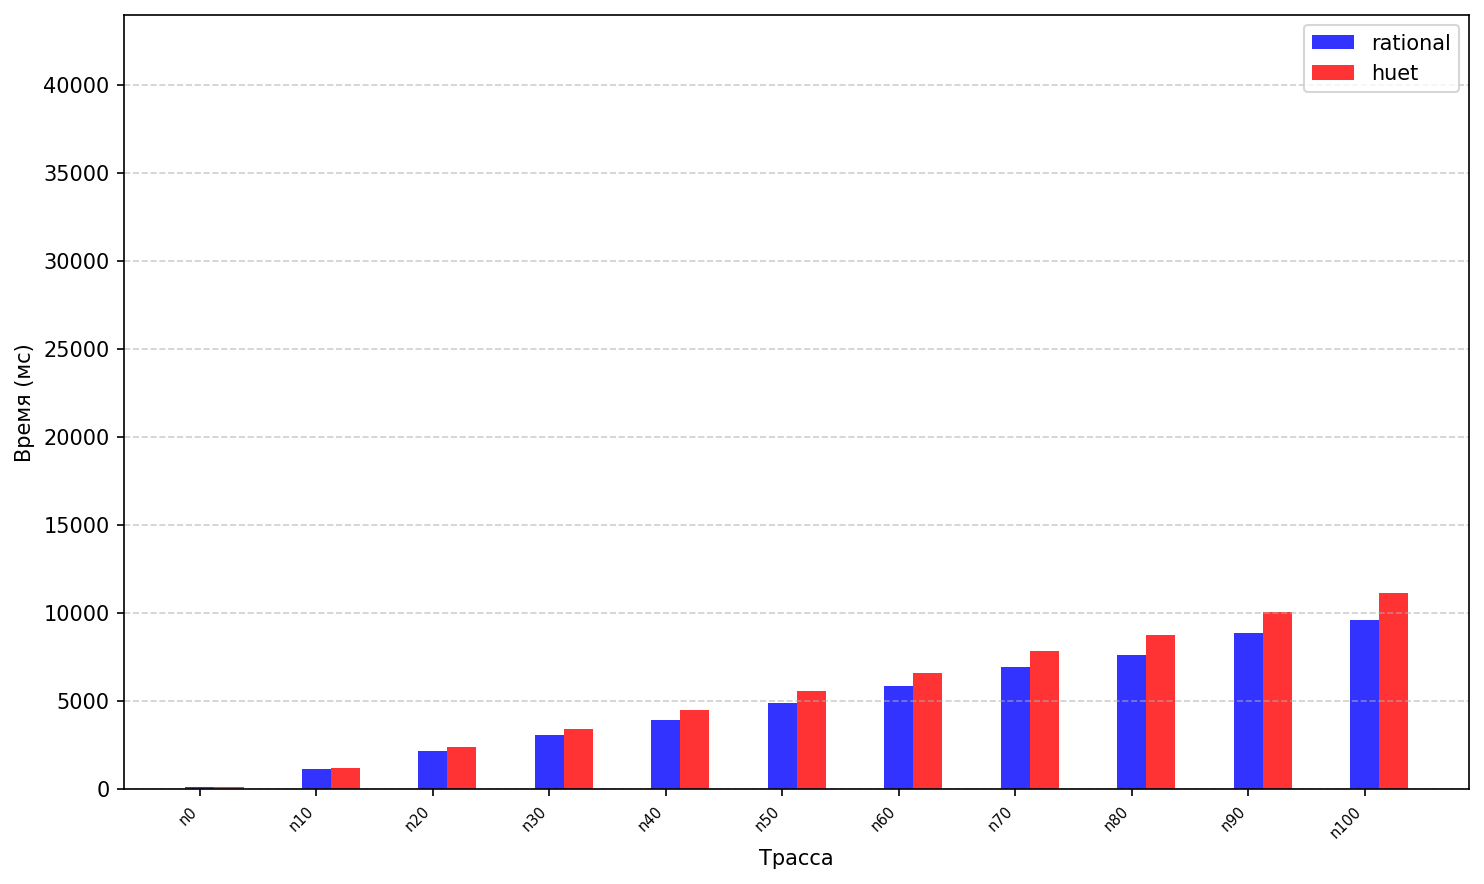
\includegraphics[width=\linewidth]{bench/ephemeral/synth_full.png}
        \subcaption{\texttt{full}}
    \end{subfigure}
    \hfill
    \begin{subfigure}{.48\linewidth}
        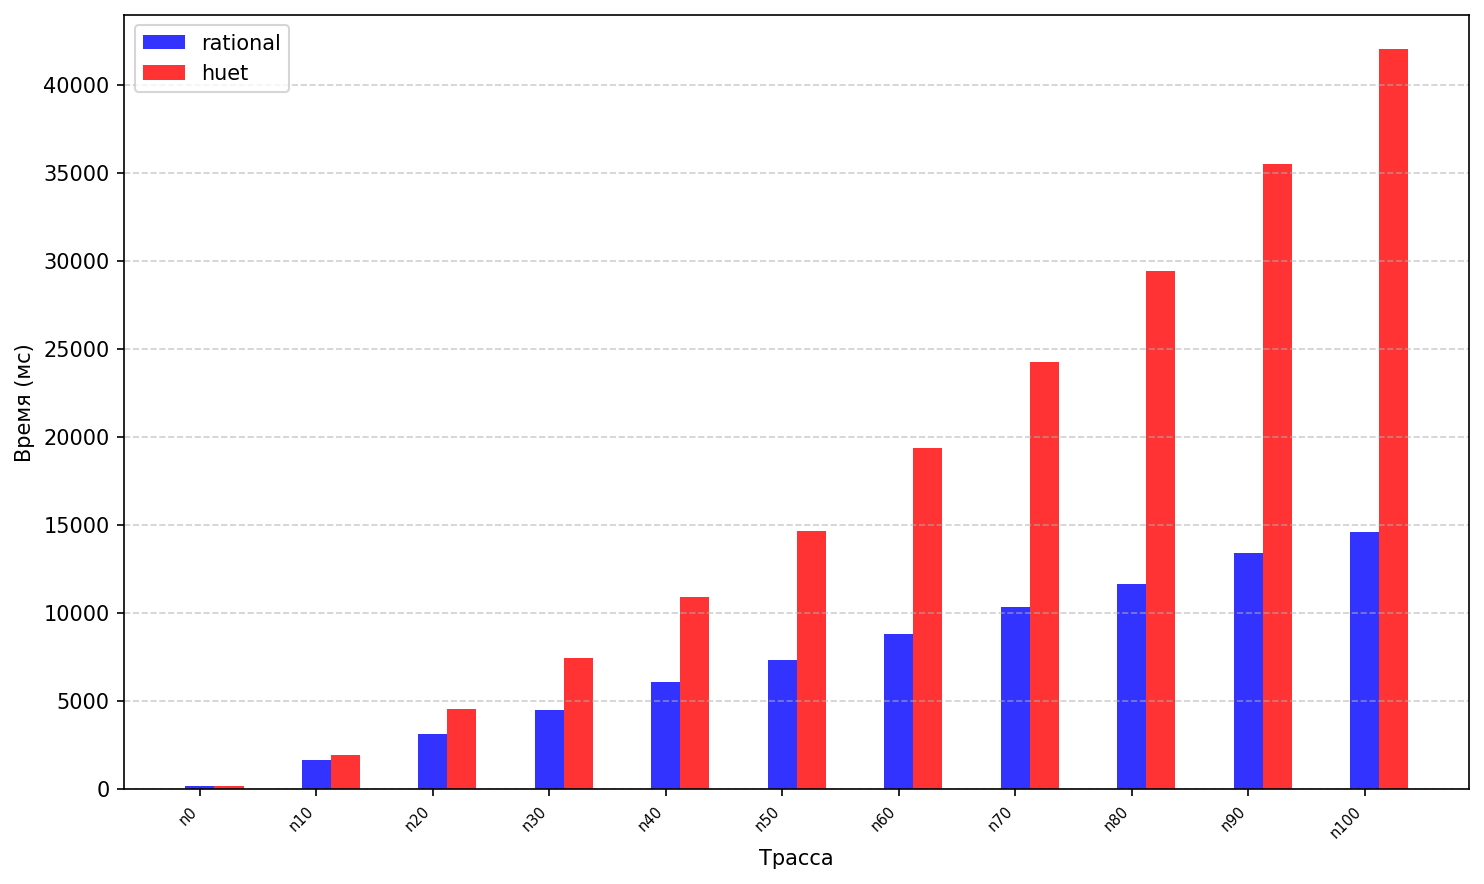
\includegraphics[width=\linewidth]{bench/ephemeral/synth_left_right.png}
        \subcaption{\texttt{left\_right}}
    \end{subfigure}
    \\
    \begin{subfigure}{.48\linewidth}
        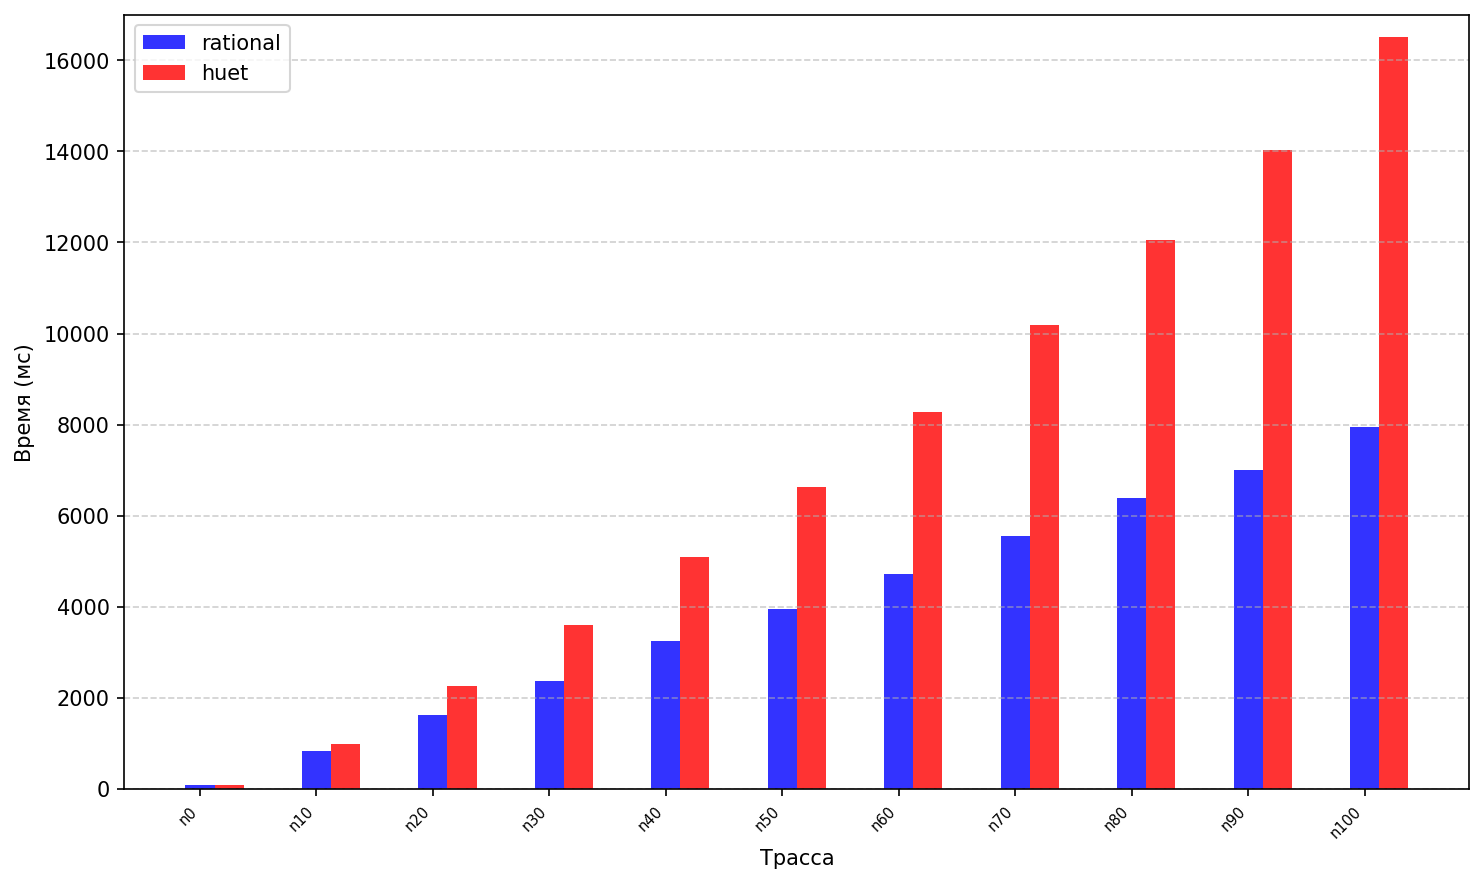
\includegraphics[width=\linewidth]{bench/ephemeral/synth_loops1.png}
        \subcaption{$\texttt{loops}_1$}
    \end{subfigure}
    \hfill
    \begin{subfigure}{.48\linewidth}
        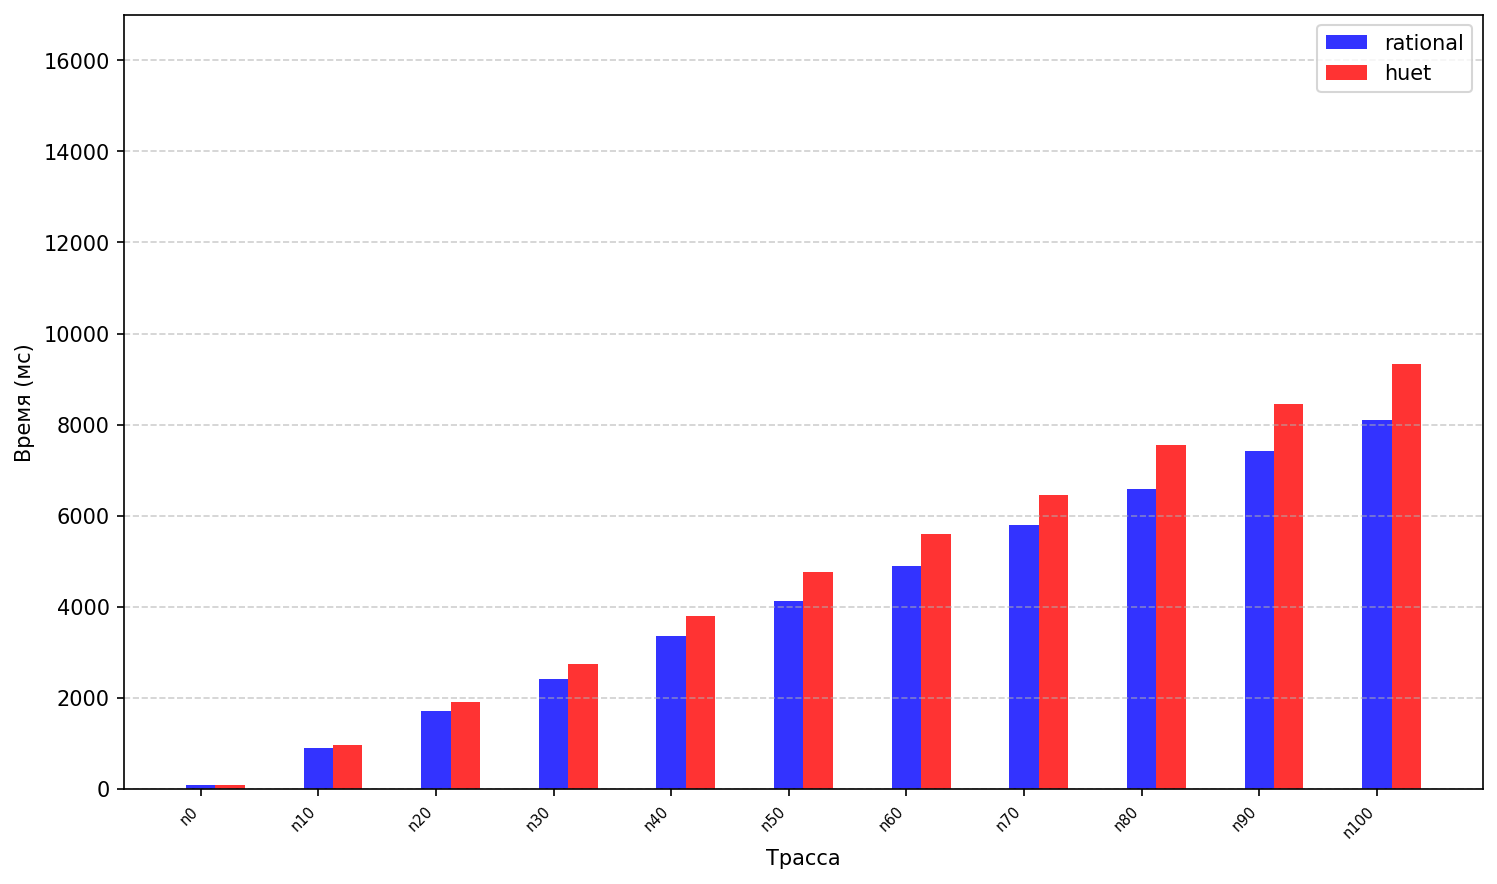
\includegraphics[width=\linewidth]{bench/ephemeral/synth_loops2.png}
        \subcaption{$\texttt{loops}_2$}
    \end{subfigure}
    \\
    \begin{subfigure}{.48\linewidth}
        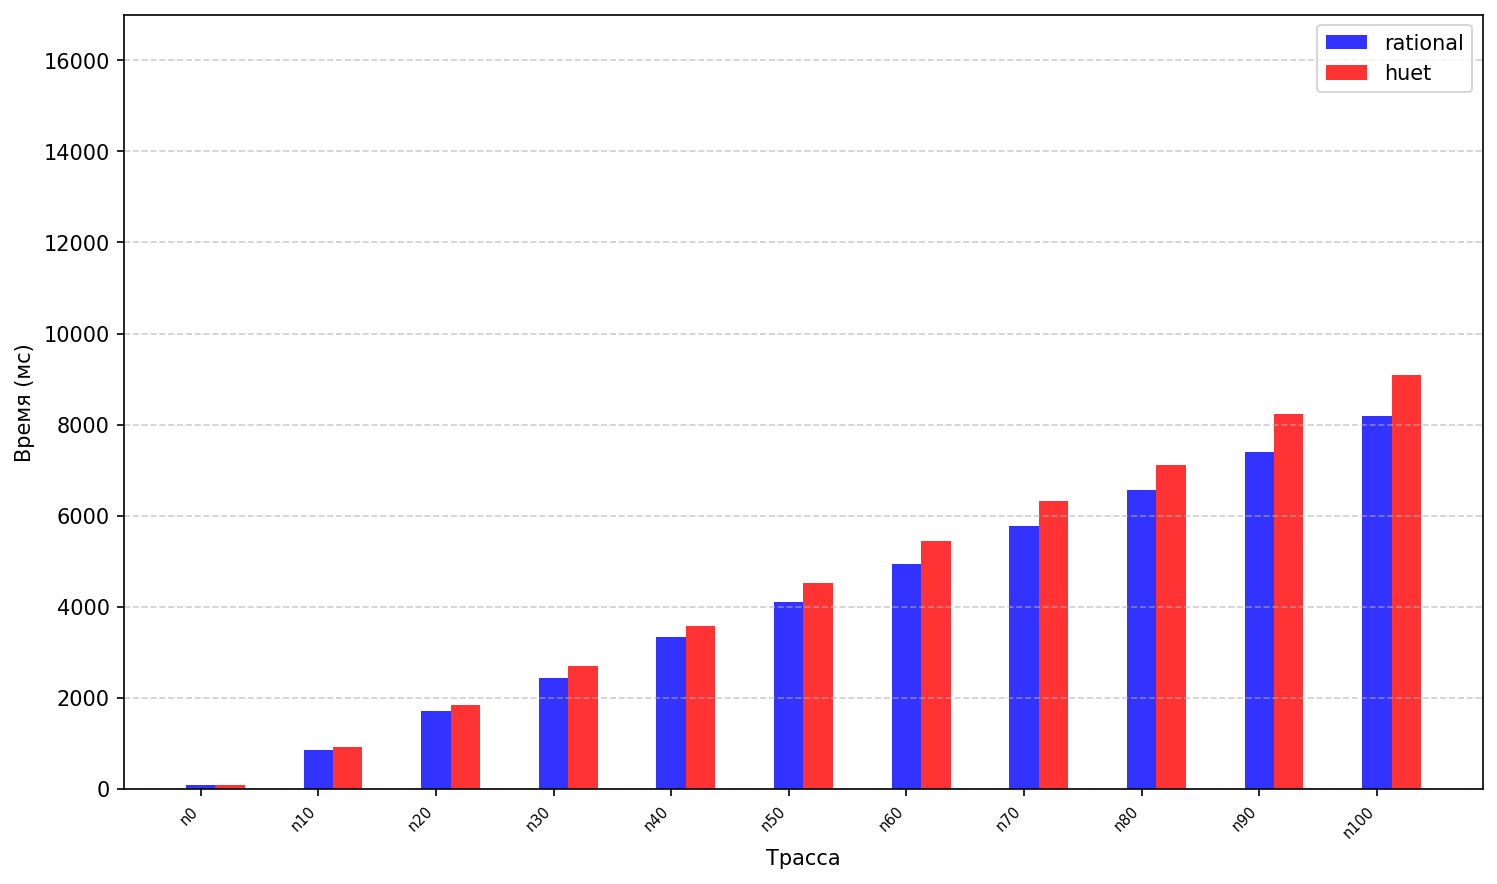
\includegraphics[width=\linewidth]{bench/ephemeral/synth_loops3.png}
        \subcaption{$\texttt{loops}_3$}
    \end{subfigure}
    \hfill
    \begin{subfigure}{.48\linewidth}
        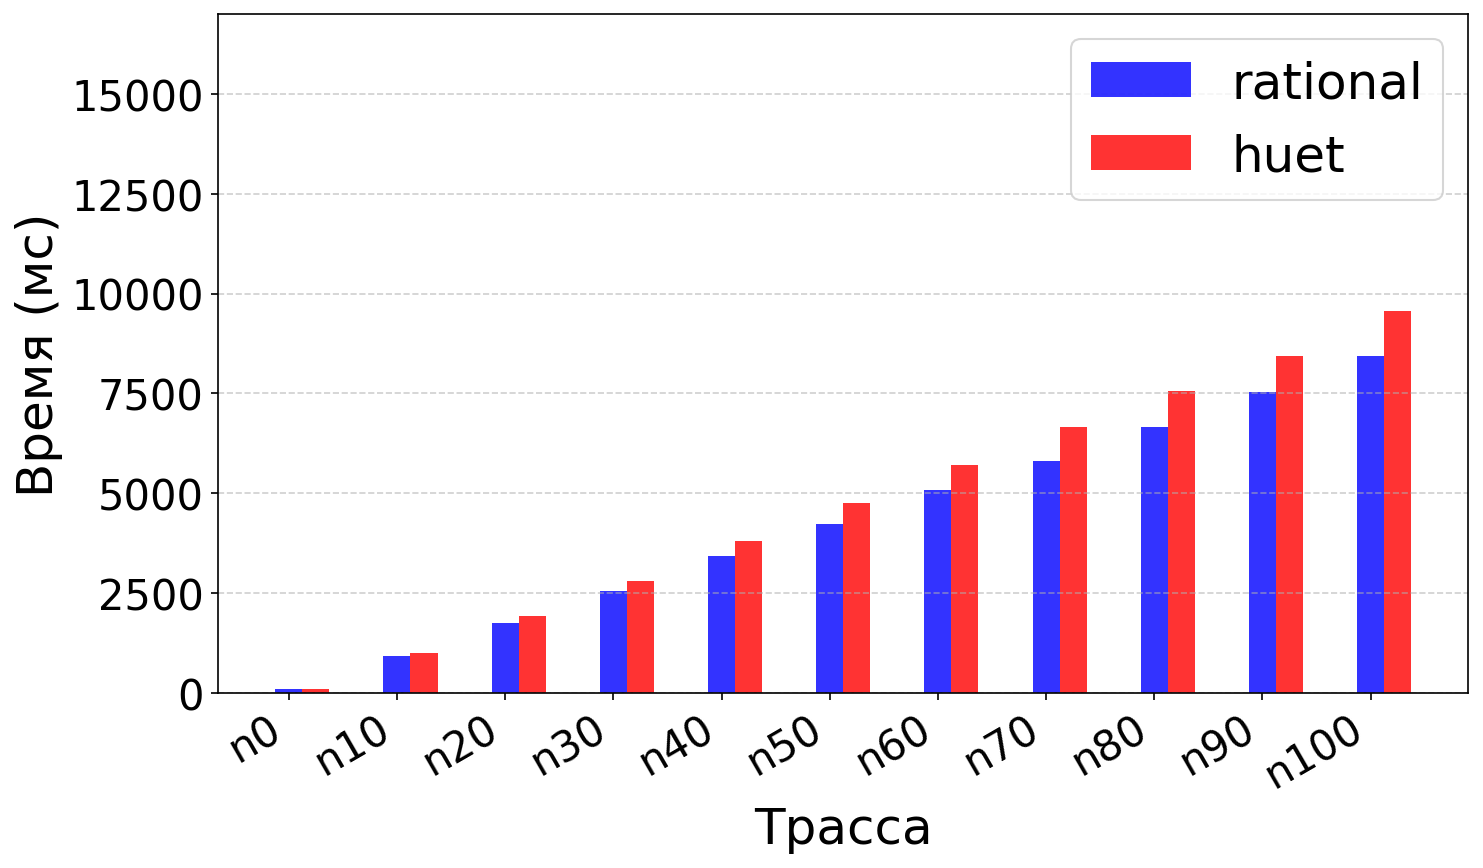
\includegraphics[width=\linewidth]{bench/ephemeral/synth_loops4.png}
        \subcaption{$\texttt{loops}_4$}
    \end{subfigure}
    \caption{Сравнение эфемерных реализаций алгоритмов рациональной унификации на синтетических тестах.}
    \label{fig:synth-ephemeral}
\end{figure}

\begin{figure}[p]
    \centering
    \begin{subfigure}{.48\linewidth}
        
\includegraphics[width=\linewidth]{bench/persistent/synth_full.png}
        \subcaption{\texttt{full}}
    \end{subfigure}
    \hfill
    \begin{subfigure}{.48\linewidth}
        
\includegraphics[width=\linewidth]{bench/persistent/synth_left_right.png}
        \subcaption{\texttt{left\_right}}
    \end{subfigure}
    \\
    \begin{subfigure}{.48\linewidth}
        
\includegraphics[width=\linewidth]{bench/persistent/synth_loops1.png}
        \subcaption{$\texttt{loops}_1$}
    \end{subfigure}
    \hfill
    \begin{subfigure}{.48\linewidth}
        
\includegraphics[width=\linewidth]{bench/persistent/synth_loops2.png}
        \subcaption{$\texttt{loops}_2$}
    \end{subfigure}
    \\
    \begin{subfigure}{.48\linewidth}
        
\includegraphics[width=\linewidth]{bench/persistent/synth_loops3.png}
        \subcaption{$\texttt{loops}_3$}
    \end{subfigure}
    \hfill
    \begin{subfigure}{.48\linewidth}
        
\includegraphics[width=\linewidth]{bench/persistent/synth_loops4.png}
        \subcaption{$\texttt{loops}_4$}
    \end{subfigure}
    \caption{Сравнение персистентных реализаций алгоритмов рациональной унификации на синтетических тестах.}
    \label{fig:synth-persistent}
\end{figure}

Основной причиной такого поведения алгоритма Юэ скорее всего является накопление классов эквивалентности между отдельными экземплярами термов-конструкторов. Теоретическое определение алгоритма предполагает, что всем таким экземплярам присвоен уникальный номер, на основе которого можно строить классы эквивалентности таким же образом, как это делает наш алгоритм с номерами переменных. Тем не менее, на практике такие номера не вводятся из-за дополнительных накладных расходов, а вместо этого они моделируются с помощью дополнительной ячейки памяти внутри объектов, в которые при необходимости записывается ссылка на другой экземпляр.

Естественно, такой подход работает довольно быстро в эфемерном случае, но приводит к увеличению последовательностей разыменования указателей. В то же время, такой подход абсолютно неприменим для персистентной реализации, что вынуждает на самом деле вводить уникальную нумерацию на объектах и поддерживать классы эквивалентности в персистентном хранилище вместе с классами эквивалентности переменных.

Помимо увеличения времени самого разыменования это приводит к увеличению размера персистентного хранилища, что, в свою очередь, замедляет и определение классов эквивалентности переменных. Дополнительным неудобством является то, что ведение нумерации само по себе добавляет накладные расходы и требует более сложной организации хранения термов в памяти.

\begin{table}[h!]
    \centering
    \begin{tabular}{l||c|c|c}
        \toprule
        \bf Алгоритм & \bf Эфемерный & \bf\makecell{Эфемерный со \\ сжатием путей} & \bf Персистентный \\
        \midrule
        Классический & 755 & 915 & \bf 1982 \\
        Наш & 847 & 727 & \bf 2155 \\
        Юэ & \bf 2677 & \bf 2651 & 62 \\
        \bottomrule
    \end{tabular}
    \caption{Число статистически значимых <<побед>> каждого алгоритма в рамках одного варианта реализации на всех трассах.}
    \label{tab:analyse}
\end{table}

Для получения более строгой количественной оценки результатов мы также оценили различия между распределениями времени работы алгоритмов на каждой трассе с помощью критерия Краскела-Уоллиса~\cite{kruskal1952use}. В случае выявления статистически значимых различий выполнялись апостериорные попарные сравнения с использованием критерия Данна~\cite{dunn1964multiple} с поправкой Бонферрони~\cite{bonferroni1936teoria}. В результате для каждой трассы было определено, какой алгоритм имеет статистически значимо меньшее время работы в рамках каждого варианта реализации. Итоговые результаты анализа приведены в \autoref{tab:analyse} в виде числа <<побед>> по каждому алгоритму в рамках одного варианта реализации.

Наконец, мы убедились в том, что сжатие путей не улучшает производительность унификации, что показано в \autoref{tab:analyse-ephemeral}.

\begin{table}[h!]
    \centering
    \begin{tabular}{l||c|c|c}
        \toprule
        \textbf{Вариант} & \textbf{Классический} & \textbf{Наш} & \textbf{Юэ} \\
        \midrule
        Эфемерный & \textbf{597} & \textbf{784} & 494 \\
        Эфемерный со сжатием путей & 470 & 345 & \textbf{685} \\
        \midrule
        Среднее отношение медиан & 1,02 & 1,00 & 1,02 \\
        \bottomrule
    \end{tabular}
    \caption{Число статистически значимых <<побед>> эфемерных вариантов реализации в рамках одного алгоритма на всех трассах.}
    \label{tab:analyse-ephemeral}
\end{table}


\section{Заключение}

В данной работе был представлен экспериментальный анализ производительности алгоритма рациональной унификации на основе алгоритма Мартелли и Росси. Было показано, что наш алгоритм превосходит по производительности широко распространённый алгоритм Юэ в персистентной реализации. К тому же, было показано, что алгоритм Юэ работает с разной скоростью на похожих входных данных (отличающихся порядком уравниваемых термов), тогда как наш алгоритм не обладает этим недостатком.

Все результаты, включая исходные коды самих алгоритмов и тестового окружения, опубликованы\footnote{\url{https://github.com/ProgMiner/rational-unification}}, что позволяет повторить проведённые эксперименты и ознакомиться с конкретными примерами реализации.


\begin{thebibliographyRU}{99}
    \Bibitem{robinson1965machine}
\by J.\,A.~Robinson
\paper {A machine-oriented logic based on the resolution principle}
\jour {Journal of the ACM (JACM)}
\publ {ACM New York, NY, USA}
\yr {1965}
\pages {23--41}
\vol {12}
\issue {1}


\Bibitem{herbrand1930}
\by J.~Herbrand
\paper {Recherches sur la théorie de la démonstration}
\publ {Impr. J. Dziewulski}
\publaddr {Varsovie}
\yr {1930}
\crossref {http://eudml.org/doc/192791}


\Bibitem{pierce2002types}
\by B.\,C.~Pierce
\book {Types and programming languages}
\publ {MIT press Cambridge}
\yr {2002}
\vol {1}
\issue {19.3}


\Bibitem{colmerauer1982prolog}
\by A.~Colmerauer
\paper {Prolog and infinite trees}
\inbook {Logic Programming}
\publ {Academic Press, Inc.}
\publaddr {USA}
\yr {1982}


\Bibitem{martelli1982efficient}
\by A.~Martelli, U.~Montanari
\paper {An efficient unification algorithm}
\jour {ACM Transactions on Programming Languages and Systems (TOPLAS)}
\publ {ACM New York, NY, USA}
\yr {1982}
\pages {258--282}
\vol {4}
\issue {2}


\Bibitem{huet1976resolution}
\by G.~Huet
\paper {R{\'e}solution d'{\'e}quations dans les langages d'ordre 1, 2, …, $\omega$}
\publaddr {Paris, France}
\yr {1976}
\crossref {http://gallium.inria.fr/~huet/PUBLIC/Huet1976.pdf}


\Bibitem{mukai1983unification}
\by K.~Mukai
\paper {A unification algorithm for infinite trees}
\inbook {Proceedings of the Eighth international joint conference on Artificial intelligence-Volume 1}
\yr {1983}
\pages {547--549}


\Bibitem{martelli1984efficient}
\by A.~Martelli, G.~Rossi
\paper {Efficient unification with infinite terms in logic programming}
\inbook {Proc. 5th Generation Computer Systems}
\yr {1984}
\pages {202--209}


\Bibitem{jaffar1984efficient}
\by J.~Jaffar
\paper {Efficient unification over infinite terms}
\jour {New Generation Computing}
\publ {Springer Science and Business Media LLC}
\yr {1984}
\pages {207--219}
\vol {2}
\issue {3}
\crossref {https://doi.org/10.1007/BF03037057}


\Bibitem{warren1983abstract}
\by D.\,H.\,D.~Warren
\paper {An Abstract Prolog Instruction Set}
\publaddr {Menlo Park, CA, USA}
\yr {1983}
\issue {Technical Note 309}
\crossref {https://www.sri.com/publication/cyber-formal-methods-pubs/an-abstract-prolog-instruction-set/}


\Bibitem{friedman2005reasoned}
\by D.\,P.~Friedman, W.\,E.~Byrd, O.~Kiselyov
\book {The Reasoned Schemer}
\publ {MIT Press}
\publaddr {Cambridge, Mass.}
\yr {2005}
\pages {169}
\totalpages {169}
\isbn {978-0-262-56214-0}


\Bibitem{kiselyov2005backtracking}
\by O.~Kiselyov, C.~Shan, D.\,P.~Friedman, A.~Sabry
\paper {Backtracking, interleaving, and terminating monad transformers: (functional pearl)}
\jour {ACM SIGPLAN Notices}
\publ {ACM New York, NY, USA}
\yr {2005}
\pages {192--203}
\vol {40}
\issue {9}


\Bibitem{baader2001unification}
\by F.~Baader, W.~Snyder
\paper {Unification Theory}
\publ {Elsevier Science Publishers B.V. and MIT Press}
\yr {2001}
\pages {445--532}
\vol {1}
\crossref {https://doi.org/10.1016/B978-044450813-3/50010-2}


\Bibitem{simon2006coinductive}
\by L.\,a.\,M.~Simon
\paper {Coinductive Logic Programming}
\inbook {Logic Programming}
\publ {Springer Berlin Heidelberg}
\publaddr {Berlin, Heidelberg}
\yr {2006}
\pages {330--345}


\Bibitem{mannila1986complexity}
\by H.~Mannila, E.~Ukkonen
\paper {On the complexity of unification sequences}
\inbook {International Conference on Logic Programming}
\yr {1986}
\pages {122--133}


\Bibitem{galler1964improved}
\by B.\,A.~Galler, M.\,J.~Fisher
\paper {An improved equivalence algorithm}
\jour {Commun. ACM}
\publ {Association for Computing Machinery}
\publaddr {New York, NY, USA}
\yr {1964}
\pages {301–303}
\vol {7}
\issue {5}
\crossref {https://doi.org/10.1145/364099.364331}


\Bibitem{lozov2023relational}
\by P.~Lozov, D.~Kosarev, D.~Ivanov, D.~Boulytchev
\paper {Relational Solver for Java Generics Type System}
\inbook {Logic-Based Program Synthesis and Transformation - 33rd International Symposium, LOPSTR 2023, Cascais, Portugal, October 23-24, 2023, Proceedings}
\publ {Springer}
\yr {2023}
\pages {118--128}
\vol {14330}
\crossref {https://doi.org/10.1007/978-3-031-45784-5_8}


\Bibitem{domoratskiy2024relational}
\by E.~Domoratskiy, D.~Boulytchev
\eprint {A Relational Solver for Constraint-based Type Inference}
\yr {2024}
\crossref {https://doi.org/10.48550/arXiv.2408.17138}


\Bibitem{kruskal1952use}
\by W.\,H.~Kruskal, W.\,A.~Wallis
\paper {Use of Ranks in One-Criterion Variance Analysis}
\jour {Journal of the American Statistical Association}
\yr {1952}
\pages {583--621}
\vol {47}
\crossref {https://api.semanticscholar.org/CorpusID:51902974}


\Bibitem{dunn1964multiple}
\by O.\,J.~Dunn
\paper {Multiple Comparisons Using Rank Sums}
\jour {Technometrics}
\yr {1964}
\pages {241--252}
\vol {6}
\issue {3}
\crossref {https://doi.org/10.1080/00401706.1964.10490181}


\Bibitem{bonferroni1936teoria}
\by C.\,E.~Bonferroni
\paper {Teoria statistica delle classi e calcolo delle probabilità}
\jour {Pubblicazioni del R Istituto Superiore di Scienze Economiche e Commerciali di Firenze}
\yr {1936}
\pages {3--62}
\vol {8}


\end{thebibliographyRU}

\begin{thebibliographyEN}{99}
    \Bibitem{robinson1965machine}
\by J.\,A.~Robinson
\paper {A machine-oriented logic based on the resolution principle}
\jour {Journal of the ACM (JACM)}
\publ {ACM New York, NY, USA}
\yr {1965}
\pages {23--41}
\vol {12}
\issue {1}


\Bibitem{herbrand1930}
\by J.~Herbrand
\paper {Recherches sur la théorie de la démonstration}
\publ {Impr. J. Dziewulski}
\publaddr {Varsovie}
\yr {1930}
\crossref {http://eudml.org/doc/192791}


\Bibitem{pierce2002types}
\by B.\,C.~Pierce
\book {Types and programming languages}
\publ {MIT press Cambridge}
\yr {2002}
\vol {1}
\issue {19.3}


\Bibitem{colmerauer1982prolog}
\by A.~Colmerauer
\paper {Prolog and infinite trees}
\inbook {Logic Programming}
\publ {Academic Press, Inc.}
\publaddr {USA}
\yr {1982}


\Bibitem{martelli1982efficient}
\by A.~Martelli, U.~Montanari
\paper {An efficient unification algorithm}
\jour {ACM Transactions on Programming Languages and Systems (TOPLAS)}
\publ {ACM New York, NY, USA}
\yr {1982}
\pages {258--282}
\vol {4}
\issue {2}


\Bibitem{huet1976resolution}
\by G.~Huet
\paper {R{\'e}solution d'{\'e}quations dans les langages d'ordre 1, 2, …, $\omega$}
\publaddr {Paris, France}
\yr {1976}
\crossref {http://gallium.inria.fr/~huet/PUBLIC/Huet1976.pdf}


\Bibitem{mukai1983unification}
\by K.~Mukai
\paper {A unification algorithm for infinite trees}
\inbook {Proceedings of the Eighth international joint conference on Artificial intelligence-Volume 1}
\yr {1983}
\pages {547--549}


\Bibitem{martelli1984efficient}
\by A.~Martelli, G.~Rossi
\paper {Efficient unification with infinite terms in logic programming}
\inbook {Proc. 5th Generation Computer Systems}
\yr {1984}
\pages {202--209}


\Bibitem{jaffar1984efficient}
\by J.~Jaffar
\paper {Efficient unification over infinite terms}
\jour {New Generation Computing}
\publ {Springer Science and Business Media LLC}
\yr {1984}
\pages {207--219}
\vol {2}
\issue {3}
\crossref {https://doi.org/10.1007/BF03037057}


\Bibitem{warren1983abstract}
\by D.\,H.\,D.~Warren
\paper {An Abstract Prolog Instruction Set}
\publaddr {Menlo Park, CA, USA}
\yr {1983}
\issue {Technical Note 309}
\crossref {https://www.sri.com/publication/cyber-formal-methods-pubs/an-abstract-prolog-instruction-set/}


\Bibitem{friedman2005reasoned}
\by D.\,P.~Friedman, W.\,E.~Byrd, O.~Kiselyov
\book {The Reasoned Schemer}
\publ {MIT Press}
\publaddr {Cambridge, Mass.}
\yr {2005}
\pages {169}
\totalpages {169}
\isbn {978-0-262-56214-0}


\Bibitem{kiselyov2005backtracking}
\by O.~Kiselyov, C.~Shan, D.\,P.~Friedman, A.~Sabry
\paper {Backtracking, interleaving, and terminating monad transformers: (functional pearl)}
\jour {ACM SIGPLAN Notices}
\publ {ACM New York, NY, USA}
\yr {2005}
\pages {192--203}
\vol {40}
\issue {9}


\Bibitem{baader2001unification}
\by F.~Baader, W.~Snyder
\paper {Unification Theory}
\publ {Elsevier Science Publishers B.V. and MIT Press}
\yr {2001}
\pages {445--532}
\vol {1}
\crossref {https://doi.org/10.1016/B978-044450813-3/50010-2}


\Bibitem{simon2006coinductive}
\by L.\,a.\,M.~Simon
\paper {Coinductive Logic Programming}
\inbook {Logic Programming}
\publ {Springer Berlin Heidelberg}
\publaddr {Berlin, Heidelberg}
\yr {2006}
\pages {330--345}


\Bibitem{mannila1986complexity}
\by H.~Mannila, E.~Ukkonen
\paper {On the complexity of unification sequences}
\inbook {International Conference on Logic Programming}
\yr {1986}
\pages {122--133}


\Bibitem{galler1964improved}
\by B.\,A.~Galler, M.\,J.~Fisher
\paper {An improved equivalence algorithm}
\jour {Commun. ACM}
\publ {Association for Computing Machinery}
\publaddr {New York, NY, USA}
\yr {1964}
\pages {301–303}
\vol {7}
\issue {5}
\crossref {https://doi.org/10.1145/364099.364331}


\Bibitem{lozov2023relational}
\by P.~Lozov, D.~Kosarev, D.~Ivanov, D.~Boulytchev
\paper {Relational Solver for Java Generics Type System}
\inbook {Logic-Based Program Synthesis and Transformation - 33rd International Symposium, LOPSTR 2023, Cascais, Portugal, October 23-24, 2023, Proceedings}
\publ {Springer}
\yr {2023}
\pages {118--128}
\vol {14330}
\crossref {https://doi.org/10.1007/978-3-031-45784-5_8}


\Bibitem{domoratskiy2024relational}
\by E.~Domoratskiy, D.~Boulytchev
\eprint {A Relational Solver for Constraint-based Type Inference}
\yr {2024}
\crossref {https://doi.org/10.48550/arXiv.2408.17138}


\Bibitem{kruskal1952use}
\by W.\,H.~Kruskal, W.\,A.~Wallis
\paper {Use of Ranks in One-Criterion Variance Analysis}
\jour {Journal of the American Statistical Association}
\yr {1952}
\pages {583--621}
\vol {47}
\crossref {https://api.semanticscholar.org/CorpusID:51902974}


\Bibitem{dunn1964multiple}
\by O.\,J.~Dunn
\paper {Multiple Comparisons Using Rank Sums}
\jour {Technometrics}
\yr {1964}
\pages {241--252}
\vol {6}
\issue {3}
\crossref {https://doi.org/10.1080/00401706.1964.10490181}


\Bibitem{bonferroni1936teoria}
\by C.\,E.~Bonferroni
\paper {Teoria statistica delle classi e calcolo delle probabilità}
\jour {Pubblicazioni del R Istituto Superiore di Scienze Economiche e Commerciali di Firenze}
\yr {1936}
\pages {3--62}
\vol {8}


\end{thebibliographyEN}

\end{document}
